\chapter{Introduction}\label{chapt:intro}

Monitoring roads is an essential element in urban planning. Almost every city is developed around centers with adequate transportation facilities. They provide infrastructural support to both the agricultural and industrial sectors of every country. Given its uses in disaster management, transportation of facilities, social interaction, it is historically proven that everything can efficiently work out if we have a proper mapped site. Mapping the roads, thus, is of utmost importance.

Historically, roads were mapped manually using approximate measures, mostly for short distances, and to help religious pilgrims navigate. With the development of automobiles, maps soon became more extensive and kept in the form of books~\cite{firstMapBooks}. These were handwritten until digital maps could be produced. With the help of GPS navigation, maps started becoming digital and electronic versions were kept. These electronic versions had many advantages over their paper counterparts. Papers would quite easily be torn or lost, and this was now no longer a bugging issue. They could be replicated easily by printers or transferring files to other supported devices.

However, most of the roads in the early days were mapped using manual techniques. Taking GPS enabled devices to mark roads is both inefficient and costly. Also, some roads are inaccessible due to various factors. To combat the individual mapping of roads, Some open crowdsourcing platforms like OpenStreetMap help people continue researching by using their data. % TODO: add link. Should add like click and go or cite it?
This successfully reduced the redundant work, but there is no way to check if the data is correct. Almost always, human errors reduce the quality of data. Millions of kilometers of roads are still left to be digitalized to be used for any activity~\cite{MapsDoneOSM}. As previous road data might have changed, completing the mapping of the remaining roads still does not guarantee us the latest report.

The computer is one piece of technology which makes our work a lot simpler. With the advent of techniques such as Machine Learning, identifying patterns to solve certain kinds of Problems has become a lot easier. This work here is an attempt to use image segmentation based on computer vision techniques to detect roads in satellite images. This will help us in reducing the manual workforce to a large extent. While road detection has been extensively documented in research papers, these papers mostly focus on identifying roads while the camera is on the road. While this has it's own uses in navigation, but using these techniques for surveying is not feasible as one will have to drive all the way, resulting in highly inefficient surveying. Some papers have tried to overcome this problem by high-resolution satellite images, but high-resolution images are quite expensive and have to be bought commercially. Another widespread problem these satellite images face is radiometric distortion. Roads of asphalt, sometimes turn from dark grey into bright white due to some reflection affecting satellite sensors. This is seen clearly is Figure~\ref{fig:sat_img_radiometric_distortion}~\cite{GF2-imageCaseStudy}.

\begin{figure}[h!]
  \centering
  \begin{subfigure}{0.48\textwidth}
    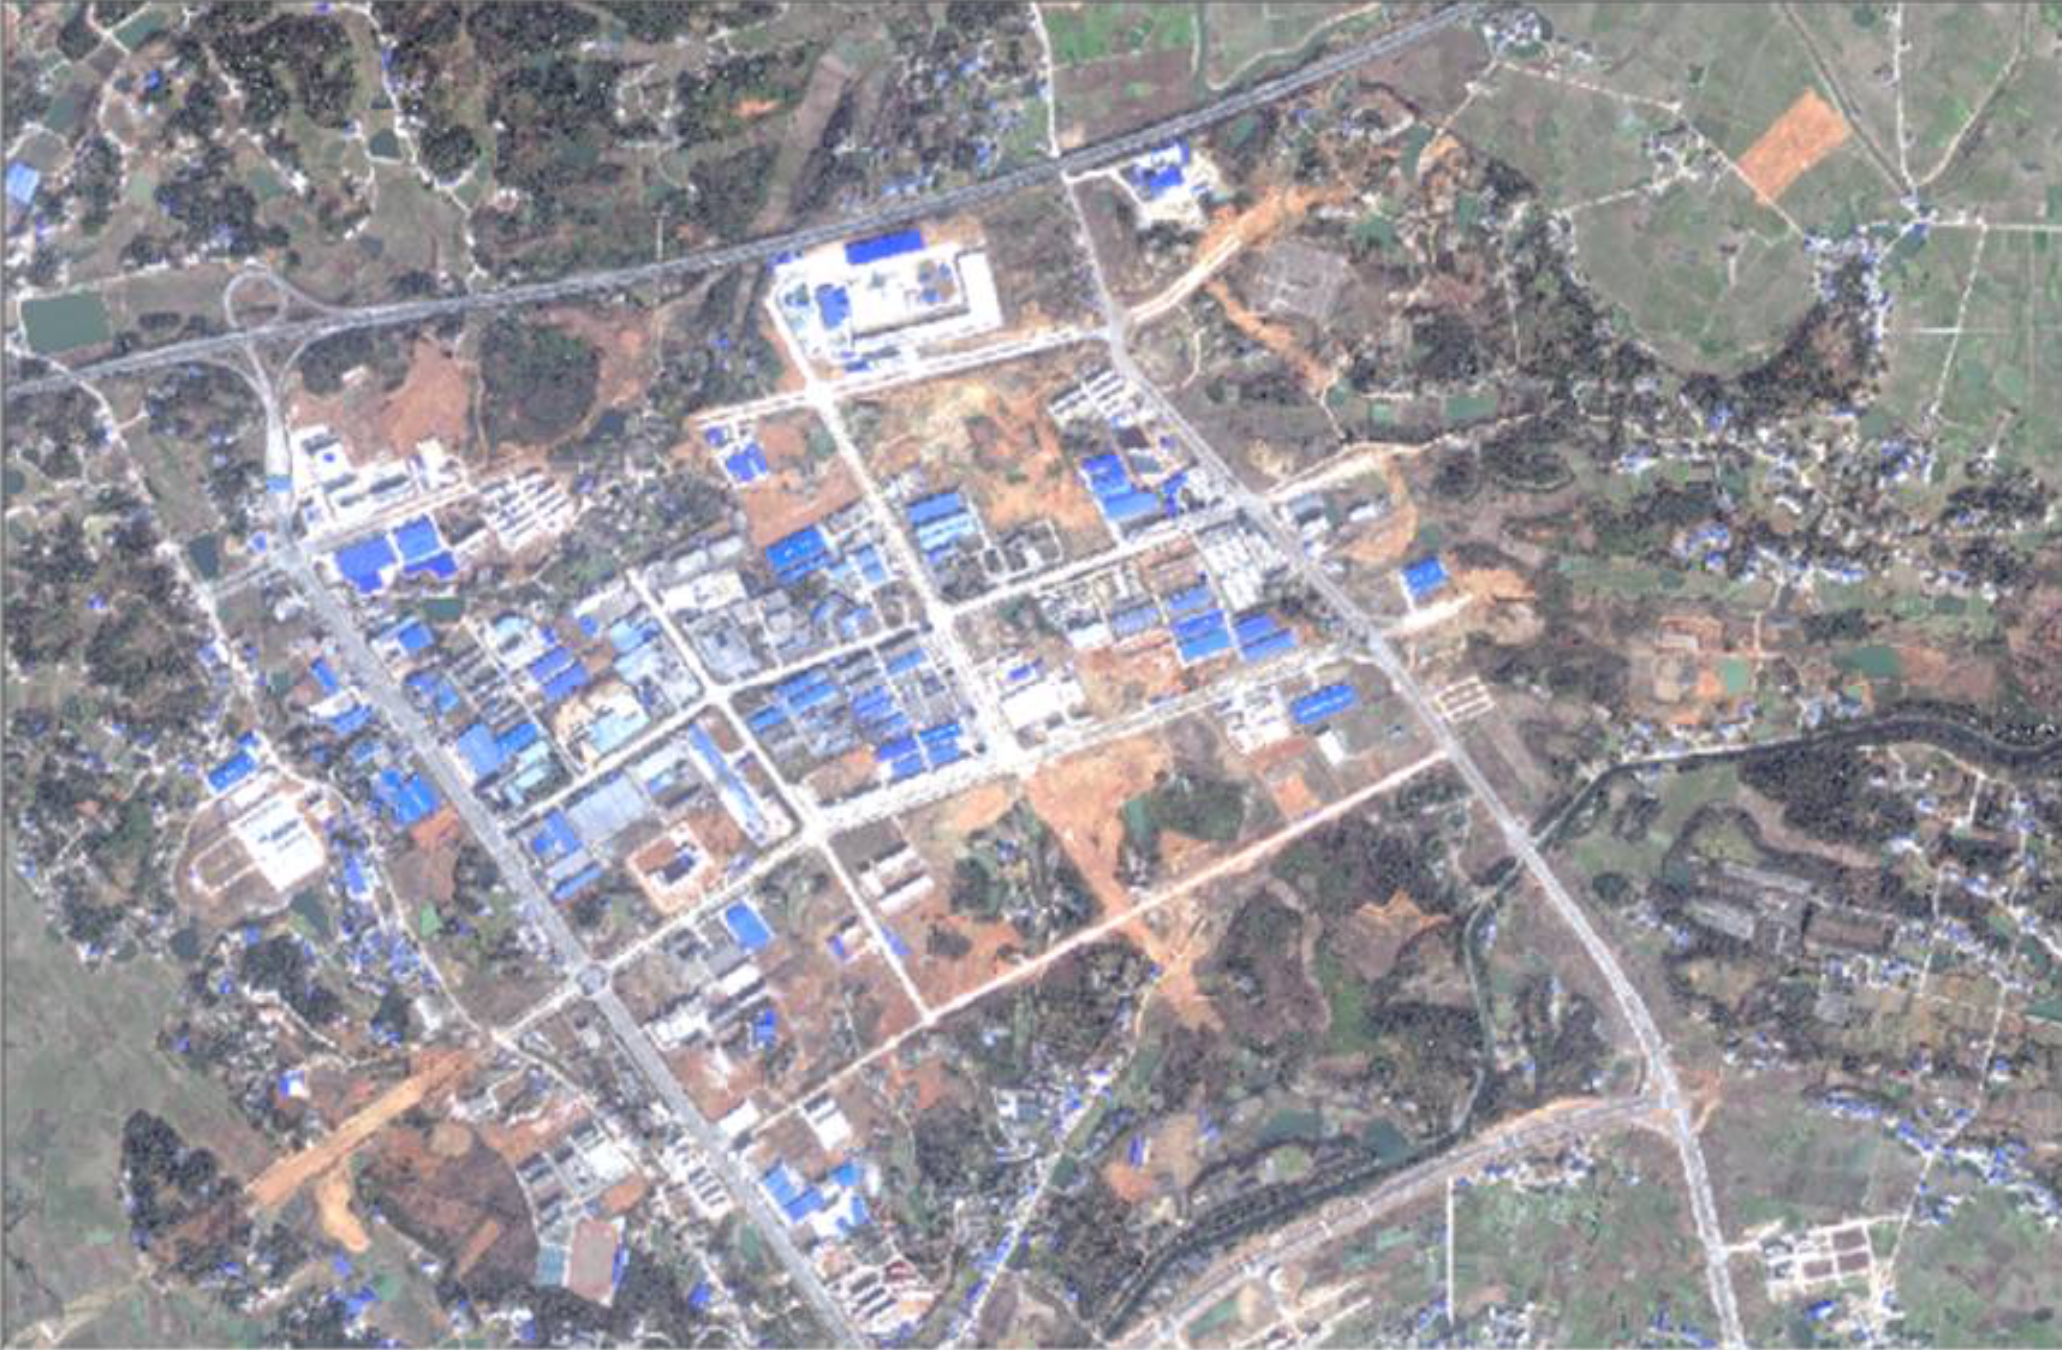
\includegraphics[width=\textwidth]{sat_img_GF2_radiometric_distortion}
    \caption{}
  \end{subfigure}~
  \begin{subfigure}{0.48\textwidth}
    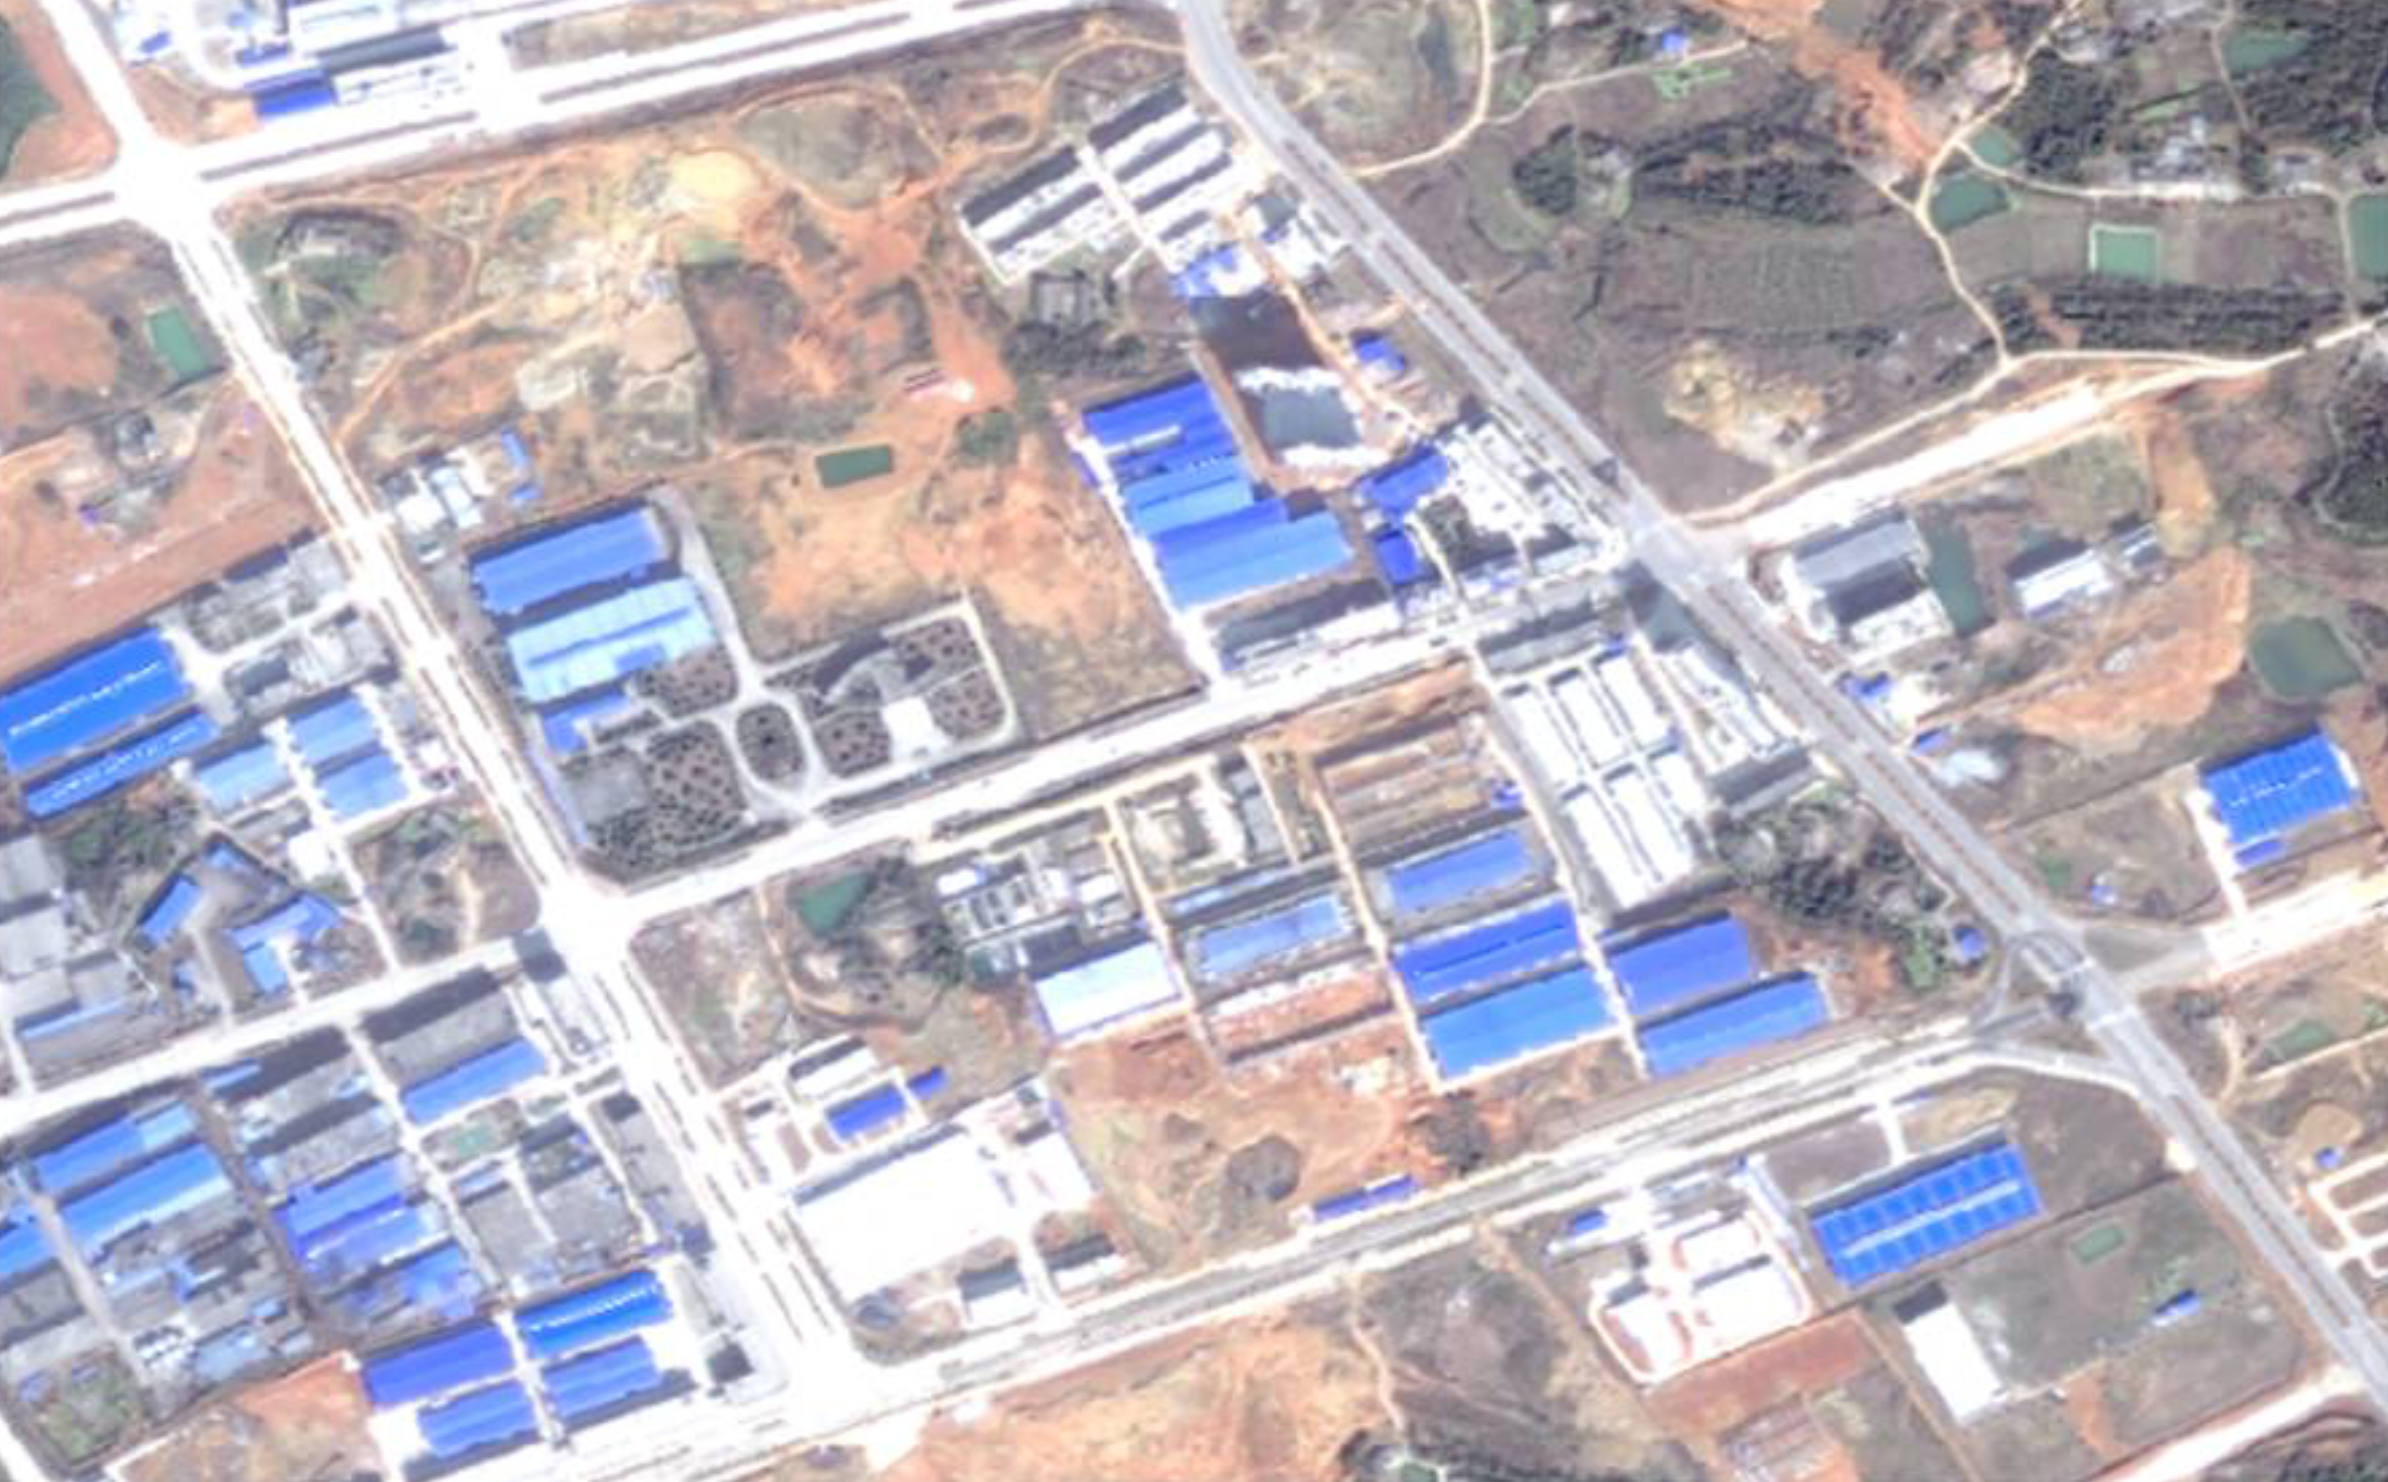
\includegraphics[width=\textwidth]{sat_img_zoomed_GF2_radiometric_distrotion}
    \caption{}
  \end{subfigure}
  \caption[Optical distortion clearly visible on roads]{Optical distortion clearly visible on roads. (a) Radiometric distortion in image from GF2 satellite (b)~Zoomed image of (a). Taken from~\cite{GF2-imageCaseStudy}.}
  \label{fig:sat_img_radiometric_distortion}
\end{figure}

Road detection using satellite data is already tough due to the many discontinuities arising given large tree canopies or due to roads being overshadowed by buildings. Road detection using a mid-resolution satellite is tougher, given the resolution is usually around 1~m-10~m. A typical two-lane road has a width of around 7~m, and this width in the best case is just depicted by just 7 pixels, leave out the worst case where a pixel hardly shows a road. This work here is an effort to use the valuable image segmentation techniques into the area of remote sensing to detect roads in mid-resolution satellite images.